\chapter{Metodologia}

Neste capítulo, serão apresentadas as técnicas utilizadas para solução do problema. O projeto 
foi realizado em um ano e sua concepção foi dividida em três frentes. São elas: desenvolvimento 
da solução para o modelo da planta, controle da planta simulada, e a implementação no dispositivo real. 
As etapas do projeto seguem abaixo:

\begin{enumerate}
 \item Desenvolvimento da solução para o modelo da planta
  \begin{enumerate}
    \item Definição e modelagem da planta de estudo.
    \item Construção do ambiente de simulação.
    \item Validação do modelo.
    \item Implementação de diferentes estratégias de controle.
  \end{enumerate}
 \item Controle da planta simulada
  \begin{enumerate}
    \item Discretização seguido da equação de diferenças da planta de estudo.
    \item Discretização seguido da equação de diferenças do controlador.
    \item Configuração do ambiente de testes com a planta rodando no computador, e o 
    controlador rodando no microcontrolador (comunicação \textit{UART}).
  \end{enumerate}
  \item Implementação no dispositivo real
  \begin{enumerate}
    \item Configuração do ambiente com a planta real e o microcontrolador (comunicação \textit{UART}).
    \item Implementação das estratégias de controle no microcontrolador e validação por meio de HIL.
    \item Implementação das estratégias de controle na planta física.
    \item Testes de validação.
  \end{enumerate}
\end{enumerate}

É importante ressaltar que a planta utilizada neste trabalho trata-se de um manipulador com três juntas
revolutas. O manipulador real, possui outras duas juntas, uma para o punho e outra para a garra, mas estas 
foram desconsideradas para a modelagem e para o controle. Este manipulador está representado na Figura \ref{fig:manipuladorRRR} e 
também é conhecido na literatura como manipulador de cotovelos (\textit{elbow manipulator}), articulado, revoluto, 
antropomórfico (\textit{anthropomorphic manipulator}), ou manipulador RRR.

\begin{figure}[ht]
  \centering
  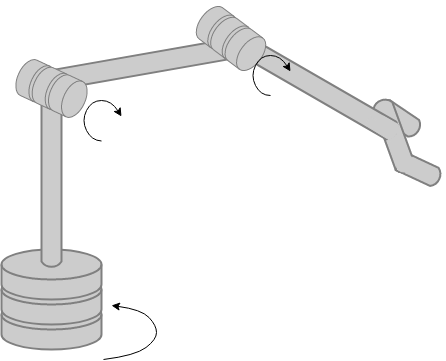
\includegraphics[width = 0.4\columnwidth]{Imagens/manipulador.png}
  \caption{Planta utilizada - manipulador de três juntas revolutas}
  \label{fig:manipuladorRRR} 
\end{figure}


\section{Desenvolvimento da solução para o modelo da planta}
\markright{\thesection ~~~ Metodologia}
\label{metodo}

A modelagem dos manipuladores robóticos visa descrever como os elos e juntas estão 
configurados fisicamente para tornar possível a configuração da orientação e posição 
deles \cite{paul1981robot}. Com isso, ao passar uma trajetória de referência para a 
entrada da planta, essa trajetória será seguida pelo sistema caso tenha algum 
controlador configurado para a planta.

No presente trabalho são realizadas duas modelagens para o manipulador: a modelagem 
cinemática e a modelagem dinâmica. A modelagem cinemática visa descrever a amplitude 
de movimento das juntas robóticas, ao passo que a modelagem dinâmica busca considerar 
as forças e torques que produzem o movimento, descrevendo, explicitamente, a relação 
entre força e movimento \cite{Spong}.

A principal ferramenta utilizada para se obter o modelo cinemático direto de um 
manipulador robótico é a convenção de \textit{Denavit-Hartenberg} \cite{paul1981robot}
. A modelagem dinâmica, por sua vez, pode ser realizada por meio das equações de 
Euler-Lagrange, que correspondem a um método baseado na energia do sistema 
\cite{Park}.

\subsection{Convenção de \textit{Denavit-Hartenberg}}
\markright{\thesubsection ~~~ Convenção de \textit{Denavit-Hartenberg}}
\label{DH}

Considera-se que o manipulador a ser modelado é de cadeia aberta, ou seja, um manipulador 
que o número de graus de liberdade seja igual ao número de articulações ativas.
Além disso, ele deve ser constituído por $n+1$ elos conectados por $n$ juntas, onde 
o elo $0$ é convencionalmente fixado ao solo. Assim sendo, segundo \citeonline{siciliano}, 
a equação cinemática direta para o manipulador pode ser calculada a partir da equação 
\ref{eq:cinematicaDireta}:

\begin{equation}
  \begin{gathered}
    T^0_n = A^0_1(q_1)A^1_2(q_2)\cdots A^{n-1}_n(q_n)
  \end{gathered}
  \label{eq:cinematicaDireta}
\end{equation}

A equação \ref{eq:cinematicaDireta} se refere à transformação de coordenadas descrevendo 
a posição e a orientação do eixo $n$ em relação à base (eixo $0$) \cite{siciliano}. Segundo
\citeonline{Spong}, na convenção DH, cada transformação homogênea $A_i$ representada na equação
\ref{eq:cinematicaDireta} equivale a um produto de quartro transformações básicas, conforme 
a equação \ref{eq:matTransHomog}:

\begin{equation}
  \begin{gathered}
    A_i = Rot_{z,\theta_i}Trans_{z,\theta_i}Trans_{x,\alpha_i}Rot_{x,\alpha_i} \\[0.5cm]
    =\begin{bmatrix}
     cos(\theta_i) & -sen(\theta_i) & 0 & 0 \\
     sen(\theta_i) & -cos(\theta_i) & 0 & 0 \\
     0 & 0 & 1 & 0 \\
     0 & 0 & 0 & 1 \\
    \end{bmatrix}
    \begin{bmatrix}
     1 & 0 & 0 & 0 \\
     0 & 1 & 0 & 0 \\
     0 & 0 & 1 & d_i \\
     0 & 0 & 0 & 1 \\
    \end{bmatrix} \\
    \times \begin{bmatrix}
     1 & 0 & 0 & a_i \\
     0 & 1 & 0 & 0 \\
     0 & 0 & 1 & 0 \\
     0 & 0 & 0 & 1 \\
    \end{bmatrix}
    \begin{bmatrix}
     1 & 0 & 0 & 0 \\
     0 & cos(\alpha_i) & -sen(\alpha_i) & 0 \\
     0 & sen(\alpha_i) & cos(\alpha_i) & d_i \\
     0 & 0 & 0 & 1 \\
    \end{bmatrix} \\[0.5cm]
    =
    \begin{bmatrix}
     cos(\theta_i) & -sen(\theta_i)cos(\alpha_i) & sen(\theta_i)sen(\alpha_i) & a_icos(\theta_i) \\
     sen(\theta_i) & cos(\theta_i)cos(\alpha_i) & -cos(\theta_i)sen(\alpha_i) & a_isen(\theta_i) \\
     0 & sen(\alpha_i) & cos(\alpha_i) & d_i \\
     0 & 0 & 0 & 1 \\
    \end{bmatrix}
  \end{gathered}
  \label{eq:matTransHomog}
\end{equation}

A matriz final encontrada na equação \ref{eq:matTransHomog} é chamada de Matriz de
Trasformação Homogênea. Os quatro parâmetros da equação \ref{eq:matTransHomog} 
representam: $a_i$ = tamanho do elo, $d_i$ = deslocamento do elo, 
$\alpha_i$ = giro do elo, $\theta_i$ = ângulo da junta. De acordo com 
\citeonline{paul1981robot}, os parâmetros são obtidos através dos itens a seguir:

\begin{itemize}
  \item Rotacionar $x_i$ em torno do eixo $z_{i}$ um ângulo $\theta_i$;
  \item Transladar ao longo do eixo $z_{i}$ uma distância $d_i$;
  \item Transladar ao longo de $x_{i+1}$ uma distância $a_i$; 
  \item Rotacionar $z_i$ em torno de $x_{i+1}$ o ângulo de torção $\alpha_i$
\end{itemize}

Assim sendo, a modelagem cinemática é obtida através da multiplicação de diversas
matrizes de transformação homogêneas individuais, conforme a equação 
\ref{eq:cinematicaDireta}. Com isso, para um manipulador com três graus de 
liberdade, a transformação de coordenadas do elemento terminal em relação a base é
dada por $T^0_3=A_1A_2A_3$ .

\subsubsection{Cinemática Diferencial e o Jacobiano}

A cinemática diferencial é responsável por fornecer a relação entre as velocidades das juntas
e a correspondente velocidade final linear e angular \cite{siciliano}. Essa relação é descrita por uma matriz, 
denominada jacobiana geométrica, que depende da configuração do manipulador. O Jacobiano Analítico, 
por outro lado, é expresso por meio da diferenciação da função cinemática direta com relação às variáveis conjuntas.
A obtenção da matriz Jacobiana é fundamental para determinar as equações de movimento do manipulador robótico.

Segundo \citeonline{Spong}, considerando um manipulador com \textit{n} graus de liberdade, a equação da cinemática direta 
pode ser escrita na forma:

\begin{equation}
  \begin{gathered}
    T^{0}_n(q) = \begin{bmatrix}
     R^{0}_n(q) & o^{0}_n(q)\\
     0 & 1\\
    \end{bmatrix}
  \end{gathered}
  \label{eq:cinematicaDireta_2}
\end{equation}

A equação \ref{eq:cinematicaDireta_2} é a mesma que \ref{eq:cinematicaDireta}, onde $q = [q_1,...,q_n]^T$ é o vetor das 
variáveis das juntas, $R^{0}_n(q)$ a matriz de rotação, $o^{0}_n(q)$ o vetor de translação, $0$ a perspectiva, e $1$ o 
fator de escala. A relação da velocidade linear $v^0_n$ e a velocidade angular $\omega^0_n$ em função das velocidades 
das juntas é linear \cite{siciliano}, e pode ser expressa por:

\begin{equation}
  \begin{gathered}
    v^0_n = J_v \dot{q}
  \end{gathered}
  \label{eq:jacob_velLinar}
\end{equation}

\begin{equation}
  \begin{gathered}
    \omega^0_n = J_\omega \dot{q}
  \end{gathered}
  \label{eq:jacob_velAngular}
\end{equation}
onde $J_v$ e $J_\omega$ são matrizes $3 \times n$. É possível ainda, reescrever as equações \ref{eq:jacob_velLinar} e
\ref{eq:jacob_velAngular} da seguinte forma:
\begin{equation}
  \begin{gathered}
    \xi = J\dot{q}
  \end{gathered}
  \label{eq:jacob_ambos}
\end{equation}

\begin{equation}
  \begin{gathered}
    \xi = \begin{bmatrix}
     v^0_n\\
     \omega^0_n\\
    \end{bmatrix}
    \quad \textrm{e} \quad 
    J = \begin{bmatrix}
     J_v\\
     J_\omega\\
    \end{bmatrix}
  \end{gathered}
\end{equation}

O vetor $\xi$ também pode ser chamado de velocidade do corpo \cite{Spong}, e é importante notar que
o ele não é a derivada de uma variável de posição. A matriz $J$ é chamado de \textbf{Jacobiano} e trata-se
de uma matriz $6 \times n$ .

Combinando a parte angular e linear, segundo \citeonline{siciliano}, a metade de cima da matriz do Jacobino é
dada por:

\begin{equation}
  \begin{gathered}
    J_{v_i} = 
      \left\{
	\begin{array}{cl}
	  z_{i-1} \times (o_n - o_{i-1}) & \text{para a $i$-ésima junta revoluta}\\
	  z_{i-1} 			 & \text{para a $i$-ésima junta prismática}
	\end{array}
      \right.
  \end{gathered}
\end{equation}

A segunda metade, ou a metade baixo da matriz do Jacobino é dada por:

\begin{equation}
  \begin{gathered}
    J_{\omega_i} = 
      \left\{
	\begin{array}{cl}
	  z_{i-1} & \text{para a $i$-ésima junta revoluta}\\
	  0 	  & \text{para a $i$-ésima junta prismática}
	\end{array}
      \right.
  \end{gathered}
\end{equation}

Juntando ambas as metades da matriz do Jacobiano obtém-se para a junta revoluta a equação \ref{eq:revolJacobiano},
e para a junta prismática a equação \ref{eq:prismaticJacobiano}:

\begin{equation}
  \begin{gathered}
    J_i = \begin{bmatrix}
     z_{i-1} \times (o_n - o_{i-1})\\
     z_{i-1}\\
    \end{bmatrix}
  \end{gathered}
  \label{eq:revolJacobiano}
\end{equation}

\begin{equation}
  \begin{gathered}
    J_i = \begin{bmatrix}
     z_{i-1}\\
     0\\
    \end{bmatrix}
  \end{gathered}
  \label{eq:prismaticJacobiano}
\end{equation}

Assim sendo, as únicas ferramentas necessárias para calcular o Jacobiano são os 
vetores unitários $z_i$ e as coordenadas das origens $o_1, ..., o_n$. As coordenadas
para $z_i$ são dadas pelos três primeiros elementos da terceira coluna de $T^0_i$, 
enquanto as coordenadas de $o_n$ são dadas pelos três primeiros elementos da quarta
coluna de $T^0_i$ . Dessa forma, apenas a terceira e quarta coluna da matriz de 
homogeneidade $T$ são necessárias para obter o Jacobiano. \cite{Spong}

\subsection{Equações de \textit{Euler-Lagrange}}
\markright{\thesubsection ~~~ Equações de \textit{Euler-Lagrange}}
\label{EL}

Com o conjunto de coordenadas generalizadas independentes $q_j$, onde $n$ 
representa os graus de liberdade do manipulador, o Lagrangiano do sistema 
é definido pela equação \ref{eq:lagrangiano} \cite{Spong}, onde $K$ representa 
a energia cinética e $P$ a energia potencial do sistema:

\begin{equation}
  \begin{gathered}
    L = K - V
  \end{gathered}
  \label{eq:lagrangiano}
\end{equation}

Segundo \citeonline{Spong}, em geral, as equações de \textit{Euler-Lagrange}
aplicadas a um sistema de $n$ coordenadas, podem ser representadas na forma da
equação \ref{eq:EL}, onde a força generalizada $\tau_i$ representa as forças 
externas e torques não deriváveis de uma função potencial:

\begin{equation}
  \begin{gathered}
    \frac{d}{dt}\frac{\partial L}{\partial \dot q_i}-\frac{\partial L}{\partial q_i} = \tau_i
  \end{gathered}
  \label{eq:EL}
\end{equation}

Conforme mostrado acima, as equações de \textit{Euler-Lagrange} podem ser 
usadas para derivar as equações dinâmicas de maneira direta. É possível computar 
esses termos para um manipulador robótico de $n$ elos através das fórmulas da 
energia cinética e energia potencial usando as variáveis da articulação 
de \textit{Denavit-Hartenberg} como coordenadas generalizadas \cite{Spong}.

\subsubsection{Energia cinética para um manipulador de $n$-elos}

Segundo \citeonline{Spong} a energia cinética é dada pela soma de dois 
termos: a energia de translação, obtida concentrando toda a massa do objeto no 
centro de massa, e a energia cinética rotacional em torno do centro de massa. 
Assim, ela pode ser dada pela equação \ref{eq:energiaCinetica}:

\begin{equation}
  \begin{gathered}
    K=\frac{1}{2}mv^Tv+\frac{1}{2}\omega^T\Gamma \omega
  \end{gathered}
  \label{eq:energiaCinetica}
\end{equation}
onde $m$ é a massa do objeto, $v$ e $\omega$ são os vetores de velocidade 
linear e angular, respectivamente, e $\Gamma$ é uma matriz simétrica $3 \times 3$ 
chamada Tensor de Inércia. O Tensor de Inércia é relacionado ao quadro de 
referência inercial do manipulador. Dessa forma, é possível 
relacionar o tensor de inércia com a matriz de rotação através de uma 
transformação de similaridade:

\begin{equation}
  \begin{gathered}
    \Gamma = RIR^T
  \end{gathered}
  \label{eq:ts}
\end{equation}
onde $I$ é uma matriz que não depende do movimento do 
objeto. Cada elemento dela é calculado através de integrais sobre as
regiões do espaço ocupados por todas as partes do corpo rígido:

\begin{equation}
  \begin{gathered}
    I = \begin{bmatrix}
     I_{xx} & I_{xy} & I_{xz}\\
     I_{yx} & I_{yy} & I_{yz}\\
     I_{zx} & I_{zy} & I_{zz}\\
    \end{bmatrix}
  \end{gathered}
\end{equation}

\begin{equation}
  \begin{gathered}
    I_{xx} = \iiint(y^2+z^2)\rho(x,y,z)dxdydz\\
    I_{yy} = \iiint(x^2+z^2)\rho(x,y,z)dxdydz\\
    I_{zz} = \iiint(x^2+y^2)\rho(x,y,z)dxdydz\\
    I_{xy} = I_{yx} = - \iiint xy\rho(x,y,z)dxdydz\\
    I_{xz} = I_{zx} = - \iiint xz\rho(x,y,z)dxdydz\\
    I_{yz} = I_{zy} = - \iiint yz\rho(x,y,z)dxdydz\\
  \end{gathered}
\end{equation}

Através do Tensor de Inércia, do jacobiano, da matriz de rotação e da massa de
cada parte do braço obtém-se a energia cinética do manipulador:

\begin{equation}
  \begin{gathered}
    K=\frac{1}{2}\dot q^T D(q)\dot q
  \end{gathered}
  \label{eq:ecMat}
\end{equation}
sendo:
\begin{equation}
  \begin{gathered}
    D(q)= \sum^n_{i=1}[m_iJ_{vi}(q)^TJ_{vi}(q)+J_{\omega i}(q)^TR_i(q)I_i(q)R_i(q)^TJ_{\omega i}(q)]
  \end{gathered}
  \label{eq:dq}
\end{equation}

\subsubsection{Energia potencial para um manipulador de $n$-elos}

A energia potencial do manipulador de $n$-elos é dada pela soma da energia
potencial individual de cada parte envolvida. A única fonte de energia potencial
do manipulador é a gravidade, e assume-se que a massa total de cada elemento 
do manipulador está concentrada no seu centro de massa.

Segundo \citeonline{Spong}, a energia potencial é uma função apenas das 
coordenadas generalizadas e não de suas derivadas, assim, a energia 
potencial depende da configuração do robô, e independe da velocidade, vide 
equação \ref{eq:enePotencial}:

\begin{equation}
  \begin{gathered}
    P = \sum^n_{i=1}P_i = \sum^n_{i=1}g^Tr_{ci}m_i
  \end{gathered}
  \label{eq:enePotencial}
\end{equation}
sendo assim, a matriz da energia potencial é dada por:
\begin{equation}
  \begin{gathered}
    g(q)=\phi_k=\frac{\partial P}{\partial q_k}
  \end{gathered}
  \label{eq:enePotencialMat}
\end{equation}

\subsubsection{Equações de movimento}

Aplicando o que foi exposto acima, as equações de \textit{Euler-Lagrange} 
\ref{eq:EL} agora podem ser expressas conforme a equação \ref{eq:EL_Final}:

\begin{equation}
  \begin{gathered}
    \sum_i d_{kj}(q)\ddot q_j + \sum_{i,j}c_{ijk}(q)\dot q_i\dot q_j + \phi_k = \tau_k \quad, \quad k=1,\dots,n
  \end{gathered}
  \label{eq:EL_Final}
\end{equation}
ou, na forma matricial:
\begin{equation}
  \begin{gathered}
    D(q)\ddot q + C(q,\dot q)\dot q + g(q) = \tau
  \end{gathered}
  \label{eq:EL_FinalMat}
\end{equation}
onde $D(q)$ e $g(q)$ representam as matrizes da energia cinética e potencial 
respectivamente, e $C(q,\dot q)$ representa uma matriz construída com os chamados
Símbolos de Chistoffel, definidos matematicamente por \citeonline{Spong} através
da equação:

\begin{equation}
  \begin{gathered}
    c_{ijk} = \frac{1}{2} \left\{ \frac{\partial d_{kj}}{\partial q_i}+\frac{\partial d_{ki}}{\partial q_j}-\frac{\partial d_{ij}}{\partial q_k} \right\}
  \end{gathered}
  \label{eq:christoffel}
\end{equation}

Como o manipulador RRR possui três juntas revolutas, e cada junta revoluta precisa de uma matriz 
$3 \times 3$, serão necessários 27 Símbolos de Chistoffel diferentes.

\section{Configuração do ambiente de simulação}

A partir dos modelos cinemáticos e dinâmicos obtidos, um ambiente de simulação é 
concebido na plataforma \textit{Simulink/Matlab} (Figura \ref{fig:plantaSimulada}). Por meio desse 
ambiente, diferentes técnicas de controle são sintetizadas e validadas para o manipulador estudado. 
Posteriormente, é feita a implementação em dispositivo físico (microcontrolador) 
dos controladores sintetizados, sendo que a validação é realizada no ambiente de simulação 
desenvolvido por meio da técnica \textit{Hardware-in-the-loop} (HIL), vide Figura 
\ref{fig:solucaoModelo}. Finalmente, a última etapa corresponde à implementação das 
estratégias de controle no manipulador robótico estudado (planta física). Como ilustrado 
na Figura \ref{fig:solucaoPlanta}, nessa etapa o microntrolador é conectado ao manipulador de 
forma a controlá-lo, fazendo-o seguir uma trajetória pré-especificada. Assim, verifica-se 
se, de fato, a resposta do sistema físico em malha fechada corresponde à resposta obtida 
por meio de simulação.

\begin{figure}[h!]
  
  \centering
  \begin{subfigure}{.5\textwidth}
    \centering
    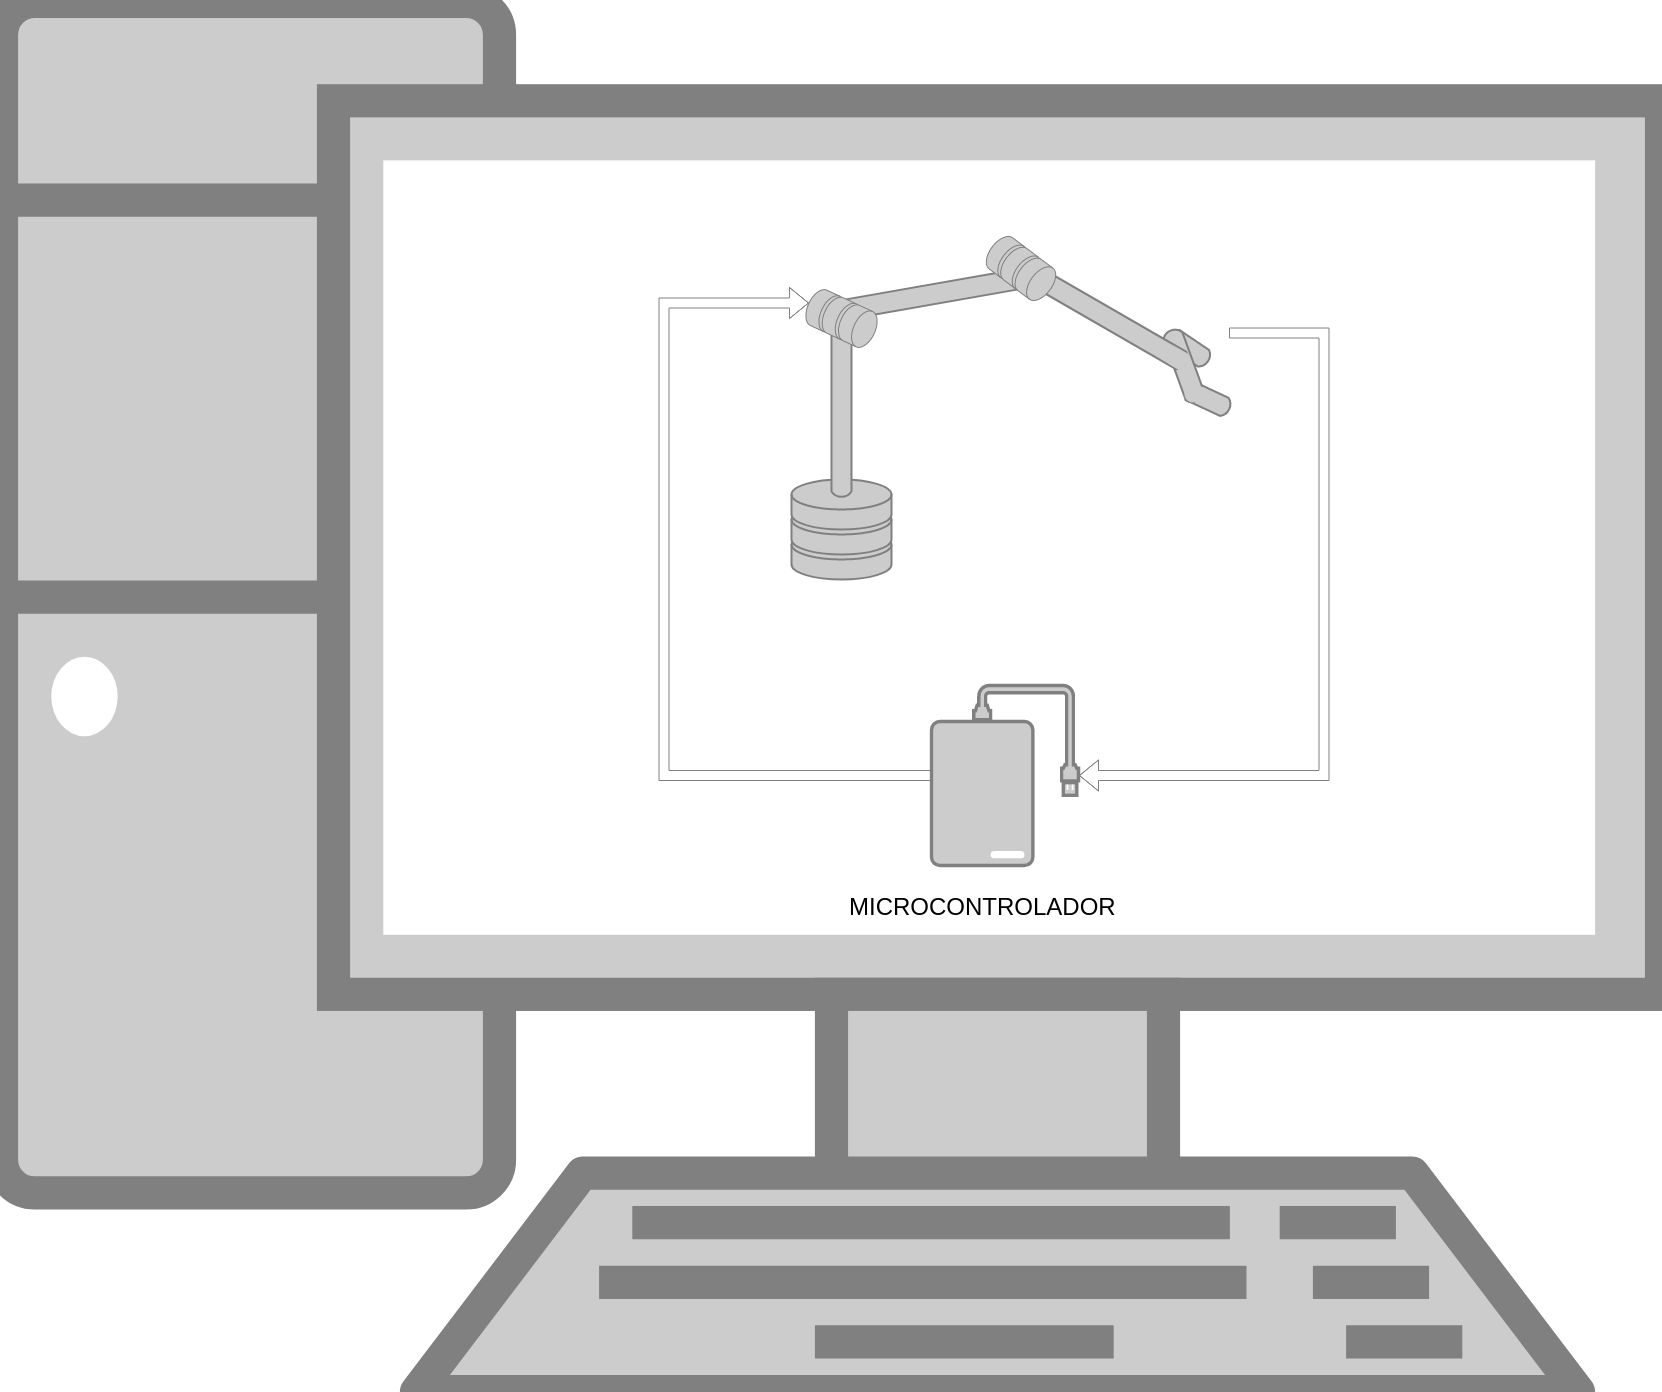
\includegraphics[width = 0.6\columnwidth]{Imagens/plantaSimulada.png}
    \caption{Planta e controlador simulados}
    \label{fig:plantaSimulada}
  \end{subfigure}%
  \begin{subfigure}{.5\textwidth}
    \centering
    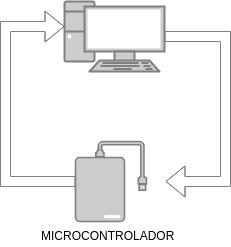
\includegraphics[width = 0.5\columnwidth]{Imagens/solucaoModelo.png}
    \caption{Solução para o modelo simulado da planta}
    \label{fig:solucaoModelo}
  \end{subfigure}%
  \\[5ex]
  \begin{subfigure}{\textwidth}
    \centering
    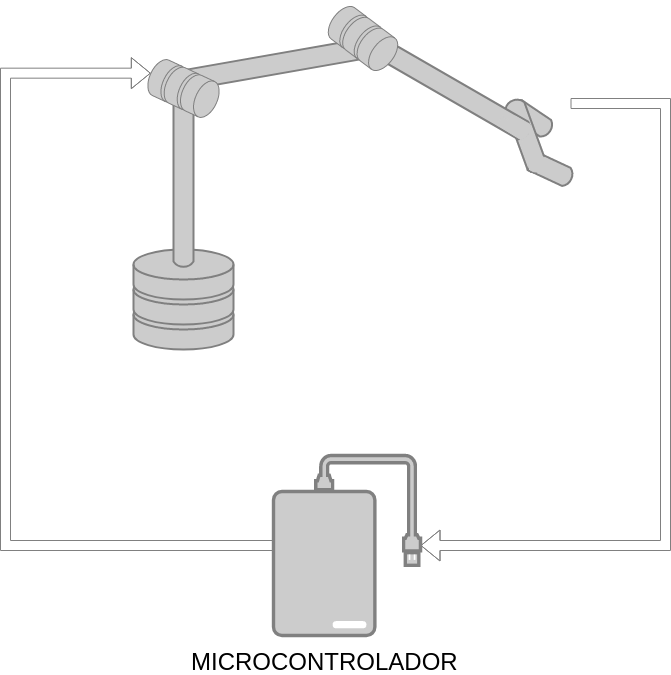
\includegraphics[width = 0.4\columnwidth]{Imagens/solucaoPlanta.png}
    \caption{Solução para a planta física}
    \label{fig:solucaoPlanta}
  \end{subfigure}%
  
  \caption{Técnica \textit{Hardware-in-the-loop} para o modelo simulado e para a planta física}
  \label{fig:simulacoes} 

\end{figure}

\section{Resumo do Capítulo}
\markright{\thesection ~~~ Metodologia}
\label{metodo1b}

Este capítulo apresentou de forma sucinta a metodologia de projeto a ser seguida para 
alcançar os objetivos propostos neste trabalho. No próximo capítulo são realizadas 
as modelagens cinemática e dinâmica do manipulador, a partir das quais o ambiente de 
simulação será construído.


\clearpage